\chapter{Literature Review}
\section{Thermocouple Array}
Few studies have proposed methods for continuous monitoring of the snowpack temperature profile. One successful instrument is the SM4 snowpack temperature and snow depth sensor. The NIVEXC is another instrument that has been used to record temperature profile measurements. Both of these systems are installed at avalanche starting zones and they measure temperature gradients using thermistors. In addition to these sensors designed for avalanche starting areas, \citet{conway_benedict_1994} created a thermistor array designed to study the infiltration of water during rain-on-snow events. 

The main objective of the SM4 \citep{ingolfsson2008sm4} is to accurately measure snow depth in avalanche starting areas. The SM4 is series of digital thermistors mounted with a fixed 20cm interval on a pole that extends through the snowpack (Fig. \ref{fig:SM4}). The SM4 Measures snow depth by identifying thermistors buried in the snow, based on damping of temperature fluctuations that is caused by the snowpack. \citep{ingolfsson2008sm4} have developed an algorithm that calculates the snow depth as a function of the temperature profile. This snow depth algorithm is proving to be more reliable than acoustic snow depth sensors because it functions during times of snowfall and ice buildup. The main challenge regarding the algorithm is greatest when the temperature of the atmosphere approaches the temperature of the snowpack. It is typically installed in avalanche starting areas where it is coupled with ultrasonic snow depth sensors for verification. Measurements are logged with a few minute interval and are regularly transferred to a central computer through wireless GSM telephone connection. In addition to snow depth, the SM4 is being used to detect and visualize high temperature gradients within the snowpack.

 \begin{figure}[!t]
    \centering
    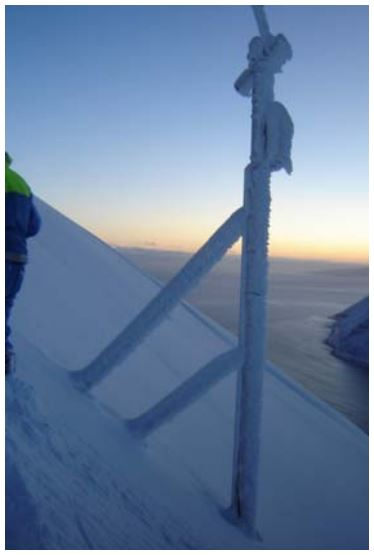
\includegraphics[width=0.8\linewidth]{figures/SM4.JPG}
    \caption{An ultrasonic sensor and a SM4 snow depth sensor covered with icing. The SM4 is attached to the upper stanchion.}
    \label{fig:SM4}
 \end{figure}
 
Like the SM4, the NIVEXC \citep{barbolininivexc} is designed to accurately measure snow depth in avalanche starting areas. The NIVEXC is an electronic snow-pole with a vertical array of sensors. It is able to record and transmit important snow cover properties, such as total snow height, snow precipitation amounts and rates, and temperature profiles. Although the SM4 and the NIVEXC both measure the temperature profile of a snowpack, their primary objective is to indirectly measure snow depth through the temperature dampening effect caused by the snowpack. One limitation of both these products is the vertical resolution, which is only 20cm. 

In \citet{conway_benedict_1994}, a rectangular grid of thermistors is used to study the infiltration of water during two midwinter rain on snow events. The progress of wetting is tracked in real time by monitoring changes in the position of the zero-degree isotherm. \citet{conway_benedict_1994} used these methods to calculate the infiltration rate and found that infiltration was not uniform. Water penetrated through localized channels that often occupied less than 50\% of the total volume of the snowpack. Their sensor was installed at 915m elevation in the Cascade Mountains near Snoqualmie Pass, Washington during 1991--1992. Measurements were made at 15-min intervals using up to 110 thermistors (Thermometrics p100DA202M) multiplexed to a data logger. The thermistors were wrapped in white heat-shrink tubing and white epoxy to make them waterproof and minimize heating from solar radiation. Each thermistor was field calibrated at the melting point for seasonal snow. Calibration was achieved at a time when the snow surrounding the thermistor was ripe and the electrical resistance of the thermistor had stabilized to a constant temperature. The temperature of ripe snow is 0\textdegree C. The temperature resolution was better than $\pm$ 0.01 \textdegree C.
 
The thermistors were arranged in a vertical, rectangular grid 1.5 m wide and up to 2 m deep. Each string consisted of 11 thermistors spaced 15 cm apart. A parallel horizontal string set at the same height 1 m away supported the leads from the thermistor beads to the multiplexer. The vertical spacing between thermistors was about 15 cm, but the thermistors were free to settle with the snowpack and the spacing decreased with time. 

Charlie Luce and Tom Black with the USFS \citep{Black_Luce} in Boise, ID constructed a thermocouple array that was installed at Bogus Basin, ID. The design for the Banner Summit Thermocouple Array is based on the thermocouple array at Bogus Basin. Charlie and Tom shared their designs and information during a meeting in October of 2018. All of the diagrams and documents that were given to us by these two can be found in Part B of the Appendix under design. 

